The tasks required in the 2016 UAV Challenge are such that a purely fixed-wing or rotor-based aircraft is unlikely to be successful; instead, teams will need to design an aircraft that make use of both flight modes. This means that last year's design, a purely fixed-wing aircraft, would not be suitable for the 2016 competition; a detailed analysis can be found in Appendix \ref{app:lastYear}.\\

As this project involves the development of a novel aircraft platform, there is scarce academic literature that is relevant to the problem at hand. This review will instead collate examples of commercial and hobby systems that were used to inspire and guide the development of the aircraft.\\

\subsection{Aircraft Design}
\todo[inline]{Do we write this section in past tense?}
\subsubsection*{Arcturus Jump}
The Arcturus Jump \cite{ref:arcturus} (Figure \ref{fig:arcturus}) is a quad-copter/fixed-wing hybrid, with propellers mounted across the wings for VTOL, and a propeller at the front for fixed-wing flight. While the design is straightforward, modifying a fixed-wing airframe to support the motors would add significant weight, decreasing thrust and maneuverability, and would also add significant drag.

\begin{figure}[!h]
	\centering
	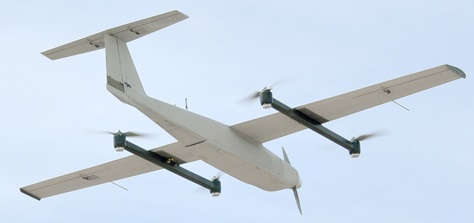
\includegraphics[width=150pt]{\IMAGEPATH /Aircraft/arcturus}
	\caption{Arcturus Jump 20}
	\label{fig:arcturus}
\end{figure}

\subsubsection*{X PlusOne}
The X PlusOne \cite{ref:xplusone} (Figure \ref{fig:xplusone}) is an incredibly fast and efficient hybrid with four front-facing propellers. It is extremely small and light, and would be relatively cheap to build, but is too small replicate with an existing airframe. Designing a new airframe would take a significant amount of time, and was outside the scope of the project.

\begin{figure}[!h]
	\centering
	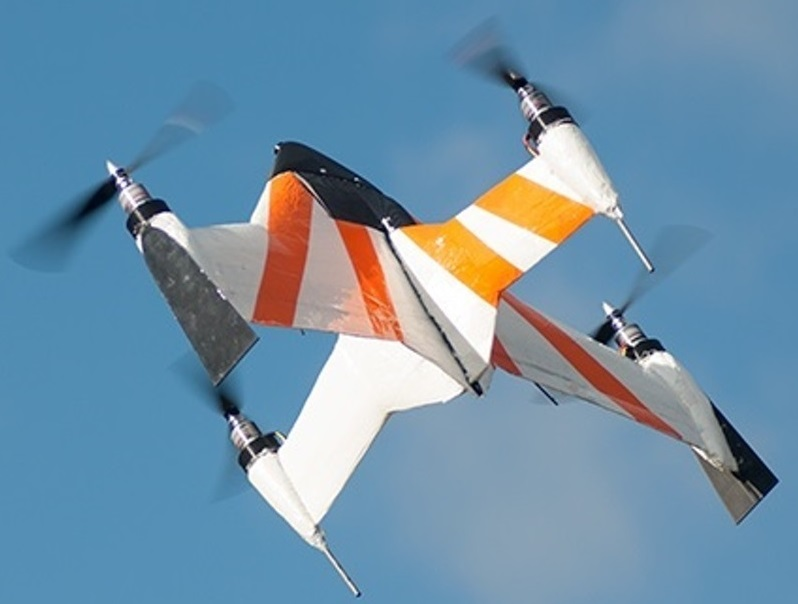
\includegraphics[width=150pt]{\IMAGEPATH /Aircraft/xplusone}
	\caption{X PlusOne}
	\label{fig:xplusone}
\end{figure}

\subsubsection*{TBS Caipirinha VTOL}
The TBS Caipirinha \cite{ref:caipirinha} (Figure \ref{fig:caipirinha}) with two front-facing propellers was also a possibility, and would require minimal modifications to existing airframes. However, developing an autonomous aircraft of this form would require the development of advanced control systems, and would result in significantly less hover maneuverability.

\begin{figure}[!h]
	\centering
	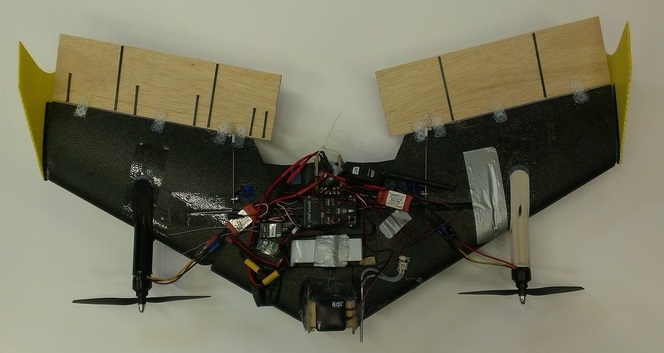
\includegraphics[width=150pt]{\IMAGEPATH /Aircraft/caipirinha}
	\caption{X PlusOne}
	\label{fig:caipirinha}
\end{figure}

\subsubsection*{FireFLY6}
Finally, the FireFLY6 \cite{ref:firefly6} (Figure \ref{fig:firefly6}) is a remote control VTOL/fixed-wing hybrid aircraft consisting of six propellers arranged in Y6 configuration, which can achieve 20-30 minutes of flight time, seven minutes of hover, and a cruising speed of 54km/h. The FireFLY6's design, and its ability to fly in VTOL or fixed-wing flight modes, make it an ideal concept for the Medical Express challenge.\\

\begin{figure}[!h]
	\centering
	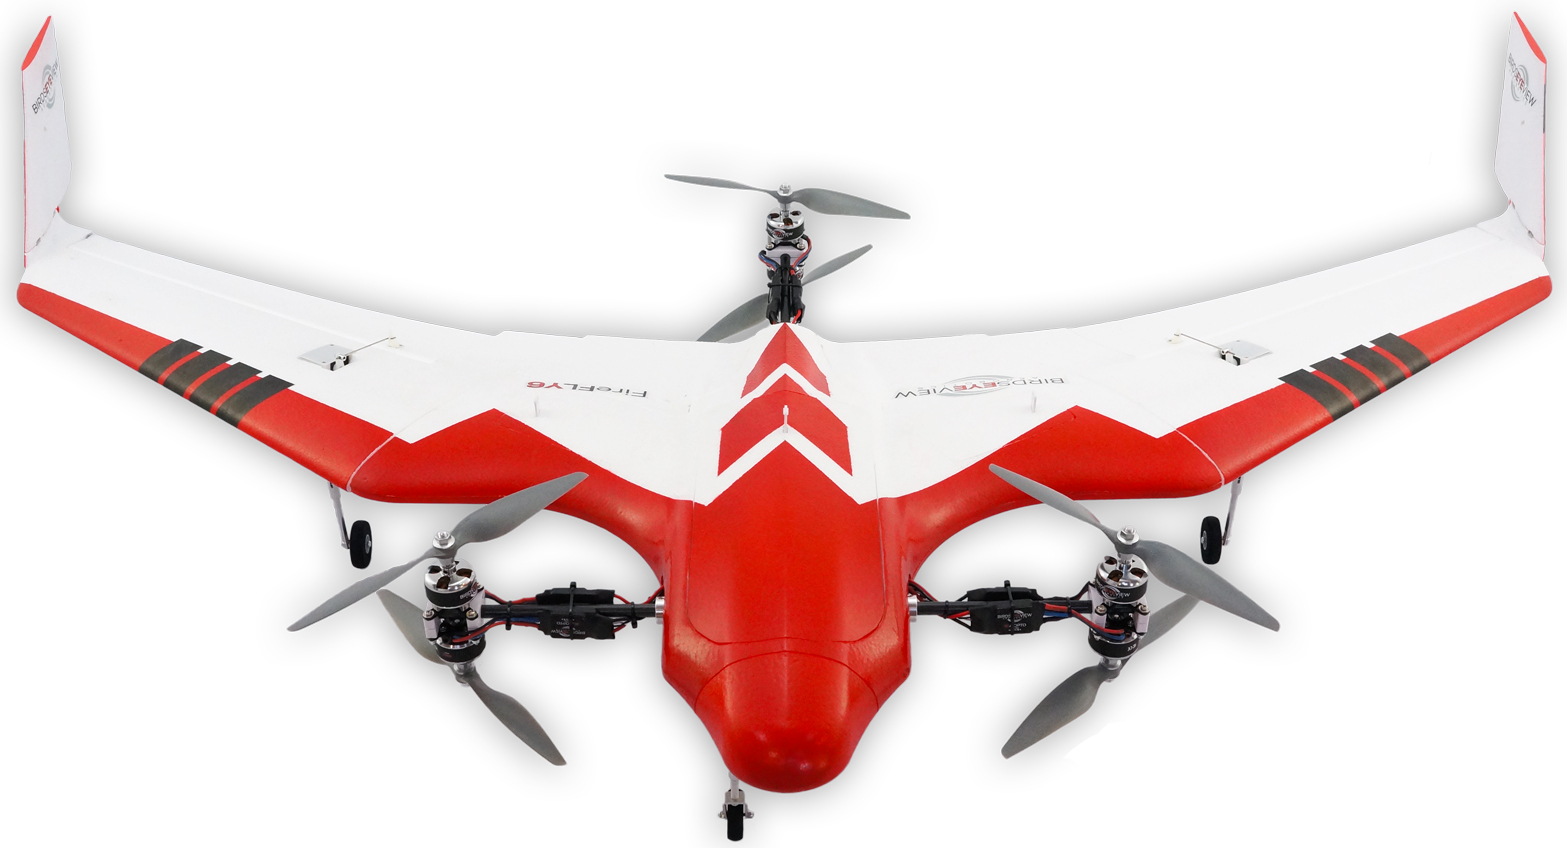
\includegraphics[width=150pt]{\IMAGEPATH /Aircraft/firefly6}
	\caption{FireFLY6}
	\label{fig:firefly6}
\end{figure}

\subsubsection*{Samsung}
INSERT STUFF HERE

\subsection{Flight Systems}
\subsubsection*{Flight Control}
The addition of a flight controller to the aircraft permits autonomous flight capabilities, including way point planning and motor control. The most viable (and well supported) options were the PixHawk \cite{ref:pixhawk}, APM 2.6 \cite{ref:ardupilot}, and PX4 \cite{ref:px4}. In order to achieve reliable and safe autonomous flight the controller must be fast and have sufficient storage for additional firmware/software to extend its capabilities. A comparison of each option may be found in \cite{ref:controller_comparison}, showing that given its larger memory storage, faster processor, and additional capabilities such as in-built gyroscopes and accelerometers, the PixHawk is the best choice for this project.

\subsubsection*{Controller Development}
The PixHawk flight controller has several flight control systems readily available, for many types of aircraft (including fixed-wing and VTOL), but as of yet has no control system that can control a hybrid aircraft. Fortunately, the PX4 autopilot (on which the PixHawk is based) is Open Source\cite{ref:ardupilotgit}, with several resources available \cite{ref:firmware1,ref:firmware2} to allow hobbyists and developers to customize the behaviour of their aircraft.

\todo[inline]{Don't really know what to do with this web page...}
\color{red}
SetUp:
http://copter.ardupilot.com/
\color{black}